To ensure that our prototype fulfills every requirements we set up in Chapter 3, we set up some testing scenarios, which we used to test the functionalities of our prototype. This scenario is made out of a maze/location like this

The table below displays how well we achieved the testing goals set by us during the problem definition. We have only managed to achieve 1 out of the 3 original requirements.
%TODO: Maybe some sort of elaboration

\begin{table}[H]
	\centering
	\begin{tabular}{|l|l|}
		\hline
		\textbf{Requirement} & \textbf{Test} \\ \hline
		The rover can be controlled using a remote device. & FAILED \\ \hline
		The rover should navigate autonomously through a maze. & FAILED \\ \hline
		The laser sensor should make a usable 2D map of its surroundings. & PASSED\\ \hline
	\end{tabular}
\end{table}
%TODO: Move this and the sentance above to the end of the chapter.

\clearpage
\section{Close proximity navigation}

The first test that was conducted on the rover, was to figure out what the measuring angle of the ultrasonic sensors are. We used the calculated blind spot distance to place an object on a piece of paper with a ruler, which was then placed beneath the rover as a guide.

\lstinputlisting[firstline=31, lastline=53, title=triple\_ultrasonic\_test.py, language=Python]{../code/autonomous-rover/triple-ultrasonic-test.py}

The code above was used to test the distance measurements from the ultrasonic sensor. As shown on figure \ref{bs-read} and \ref{bs-test}, an object on the ruler was moved back and forth to find out where the point was just before the ultrasonic sensor would pick up the object.

\begin{figure}[H]
	\centering
	\begin{subfigure}[H]{0.4\textwidth}
		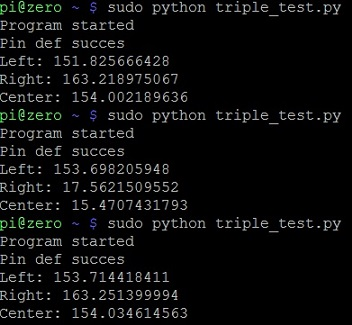
\includegraphics[width=\textwidth]{images/test-blindspotcmd.jpg}
		\subcaption{Blind spot readings}
		\label{bs-read}
	\end{subfigure}%
	\quad
	\begin{subfigure}[H]{0.5\textwidth}
		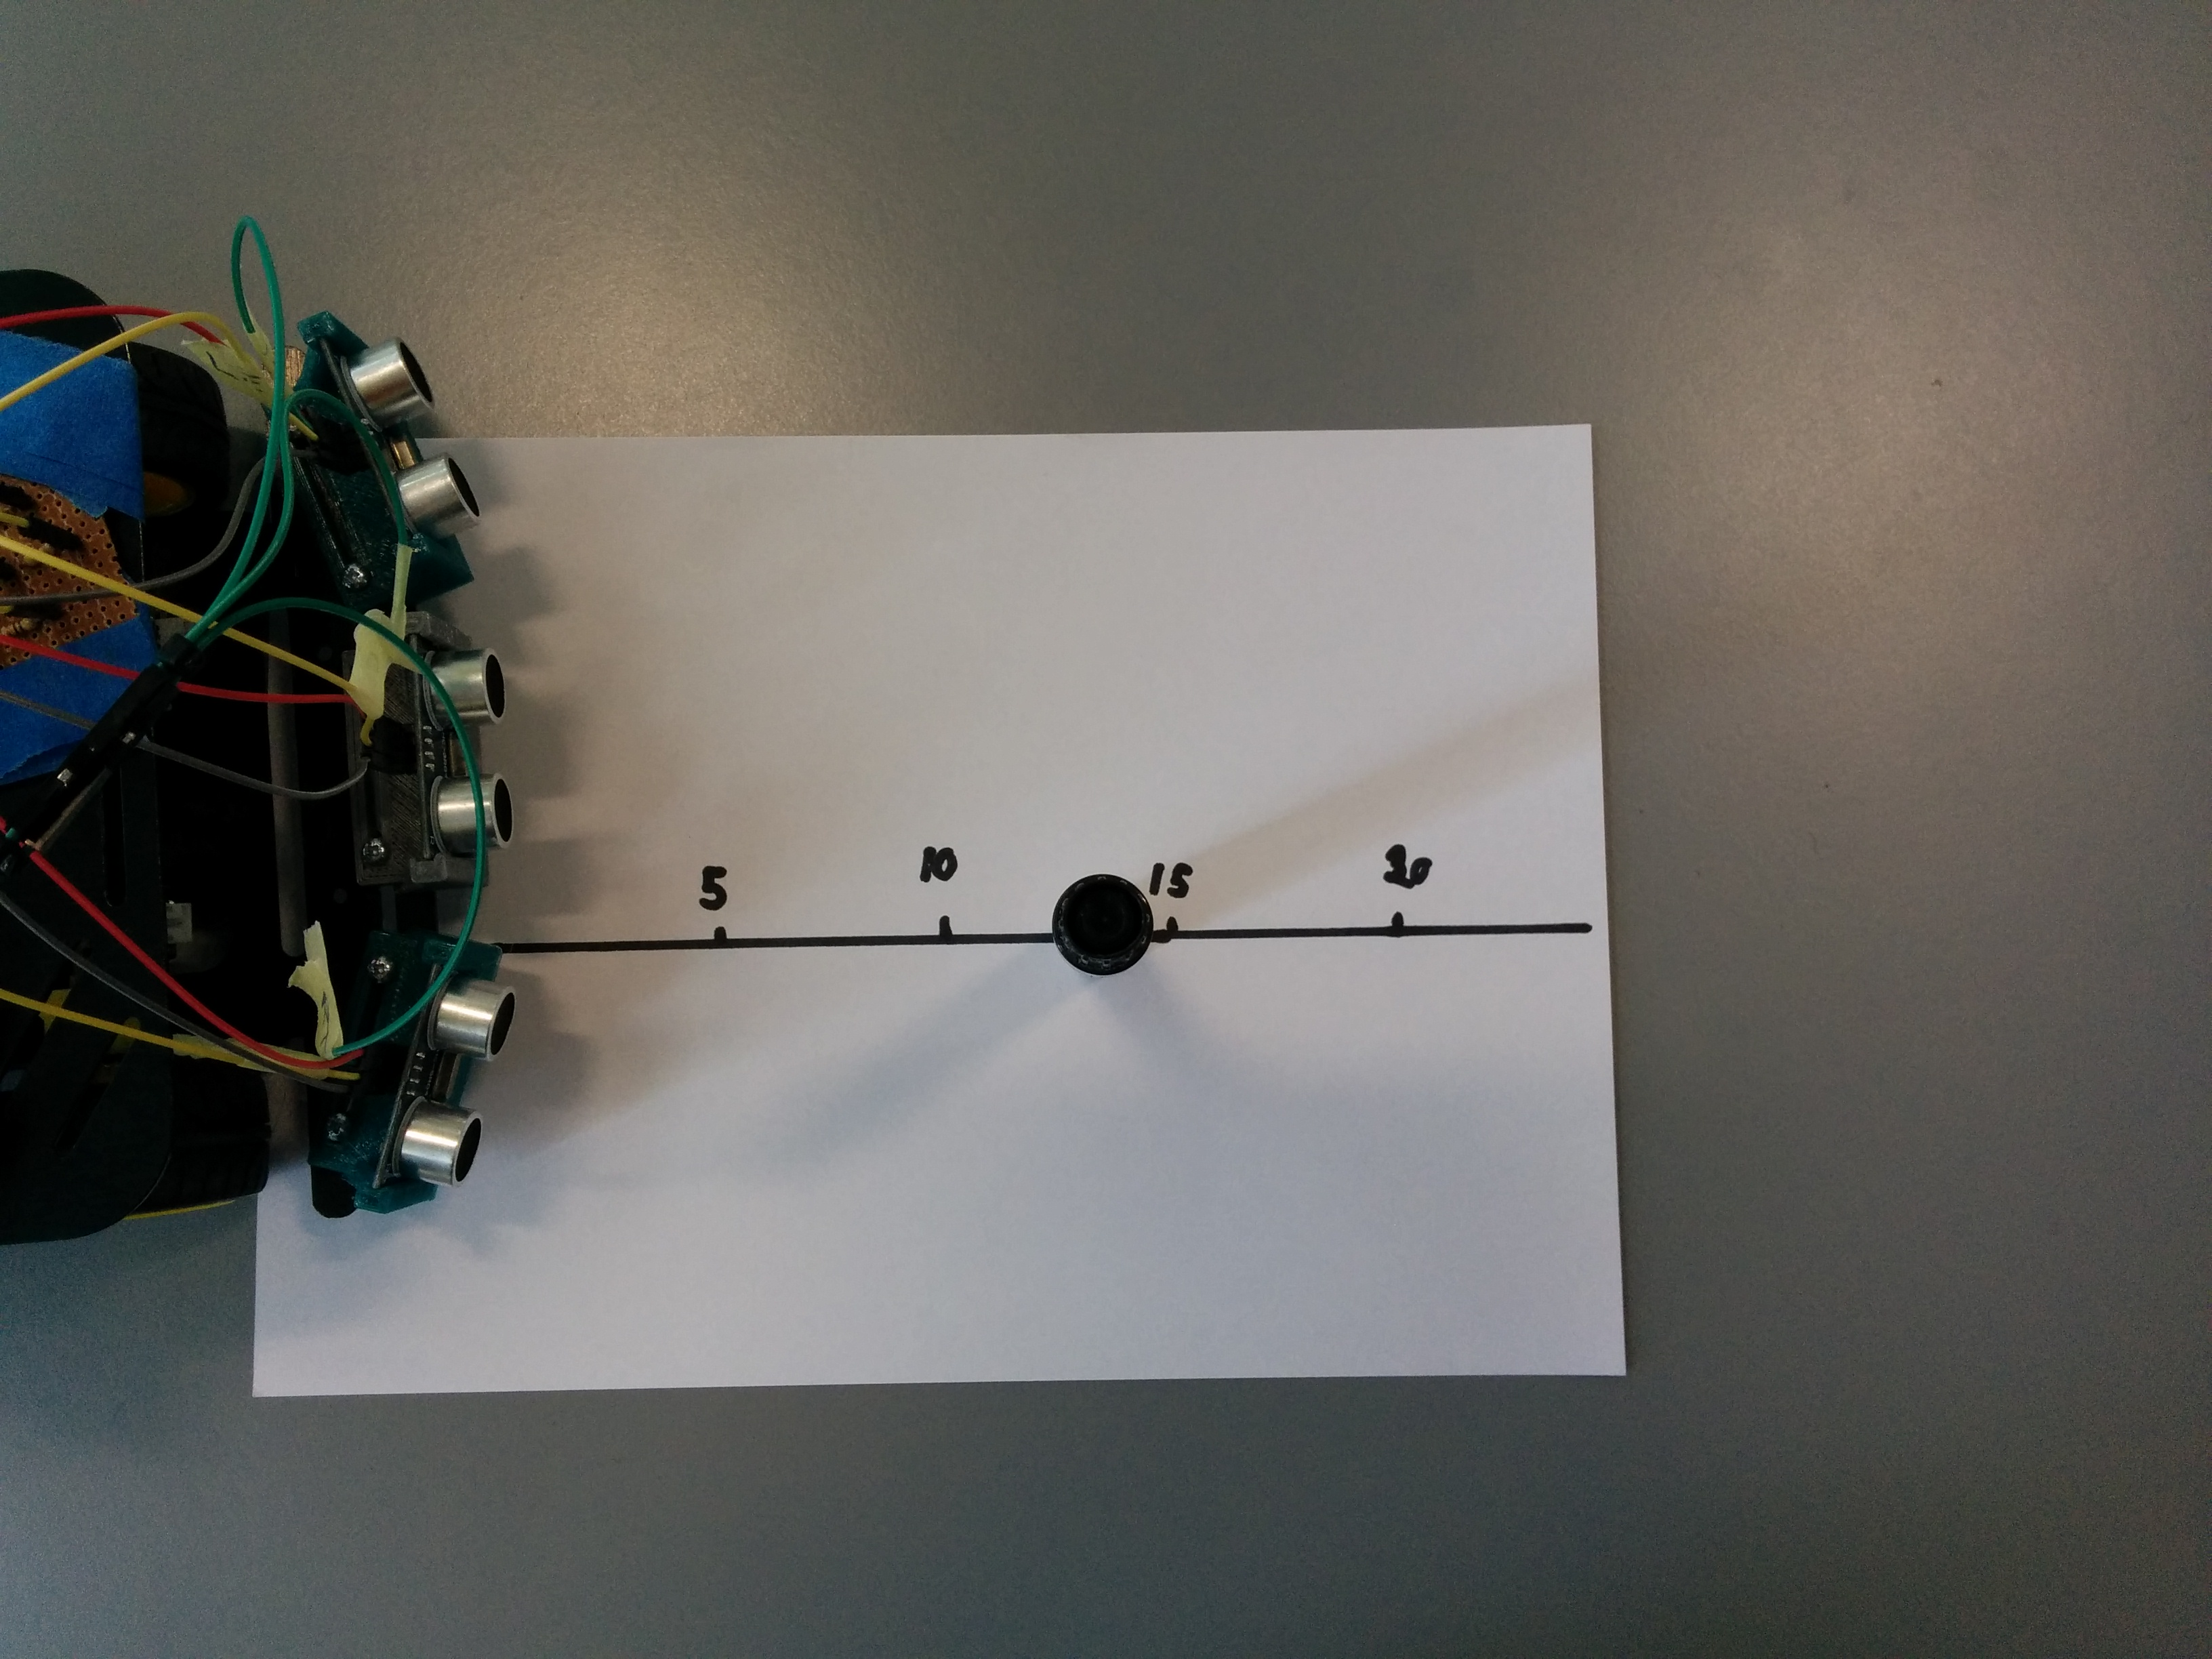
\includegraphics[width=\textwidth]{images/blindspot_test.jpg}
		\subcaption{Measuring the blind spot}
		\label{bs-test}
	\end{subfigure}%
	\quad
\end{figure}


Through testing we determined that the tipping point for the blind spot was at around 15cm. If the object used for the testing had been smaller in diameter, it would have been possible to get closer to the theoretical calculation (which is 19.8cm). Since the tipping spot was at length greater than 7.5cm (from figure \ref{calculationdiagram}, this then means that the ultrasonic sensors used for the particular project has a measuring angle of $15\degree$. \\

\begin{figure}[H]
	\centering
	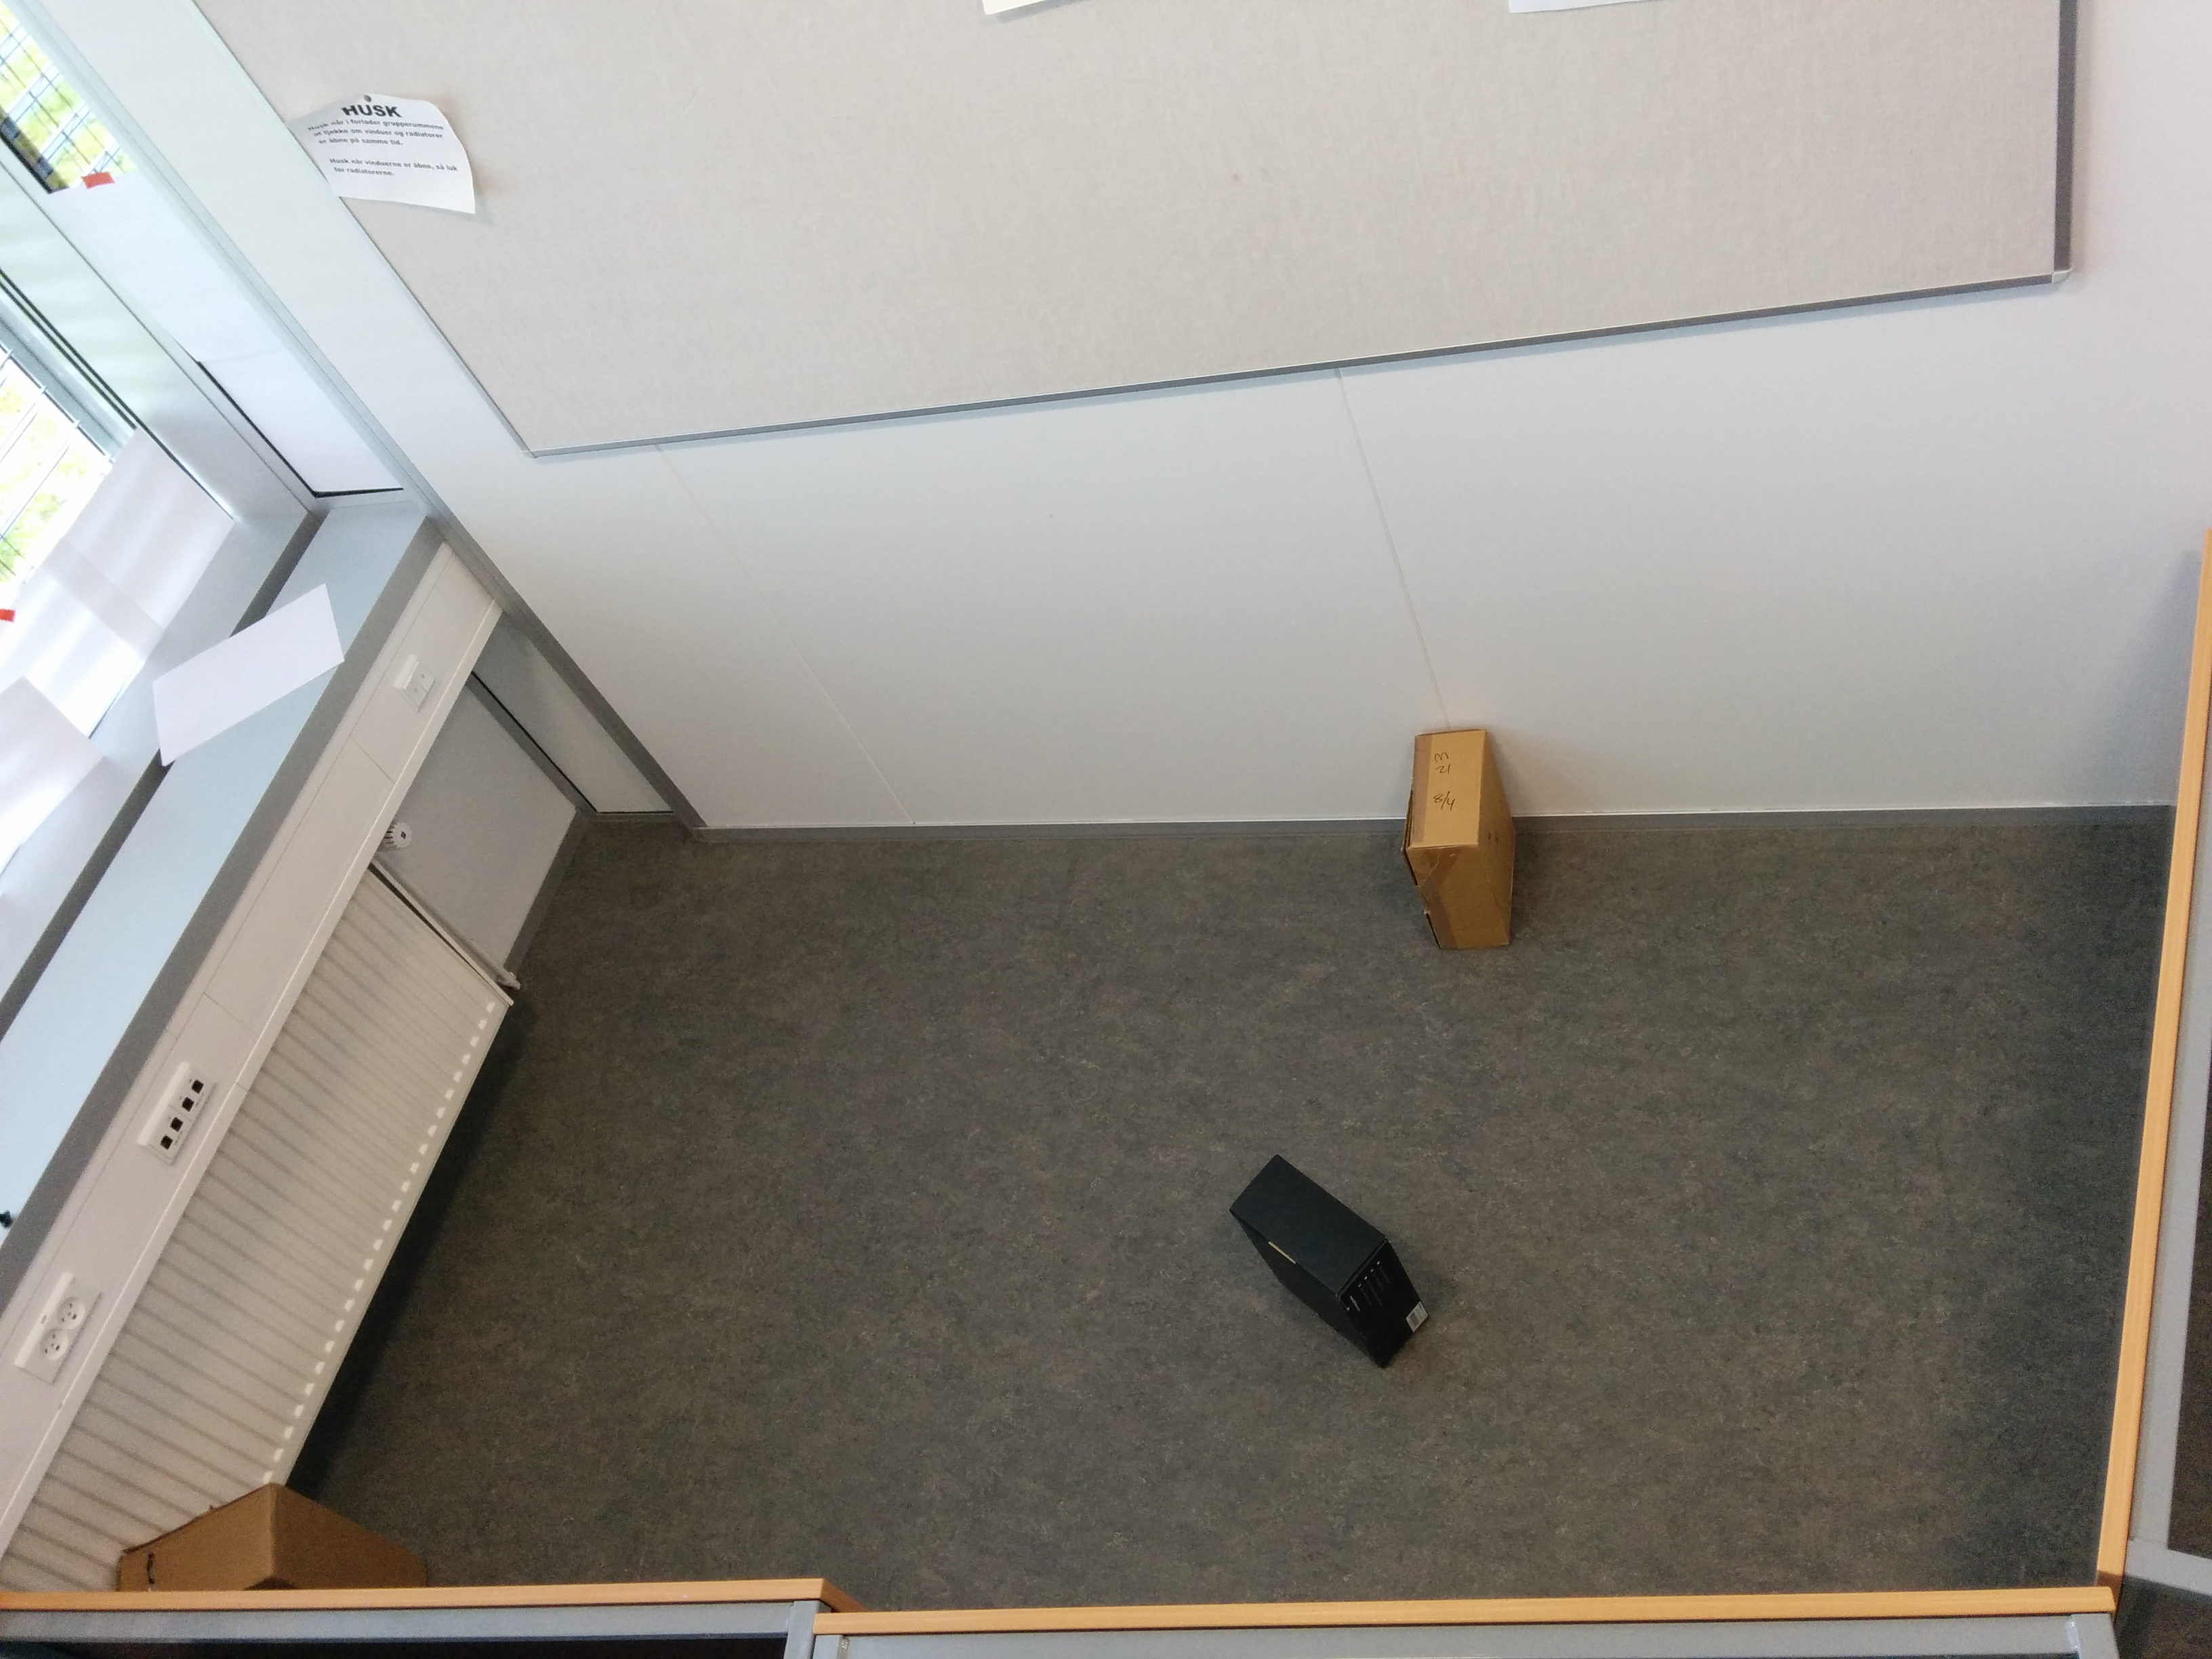
\includegraphics[width=0.6\textwidth]{images/testing-course.jpg}
	\caption{The testing course}
	\label{testcourse}
\end{figure}

The testing course had been created arbitrarily, with the purpose of placing some random objects for the rover to detect, avoid and navigate around.\\
The rover was tested using different threshold distances, which means that the rover will sense objects and walls according to that set threshold. When the distance was set to a lower length (e.g. 20cm), the rover would get really close to objects before determining a new path, this occasionally also led to the rover hitting some of the objects or the walls of the test course. If the distance threshold is set to a higher value (e.g. 50cm), the rover has an easier time navigating/avoiding objects in its path, the downside is though that with such a great distance, the rover never reaches certain parts of the course, because it often detects too many nearby objects and therefore never approaches certain areas. The rover would also sometimes get stuck in the middle of an open space, oscillating  left and right whilst slowly moving forward, the cause of this is because each time the the rover turned in one direction the rover detected a new object within a short distance, and immediately turns again - continuing in an endless loop.

\begin{figure}[H]
	\centering
	\begin{subfigure}[H]{0.4\textwidth}
		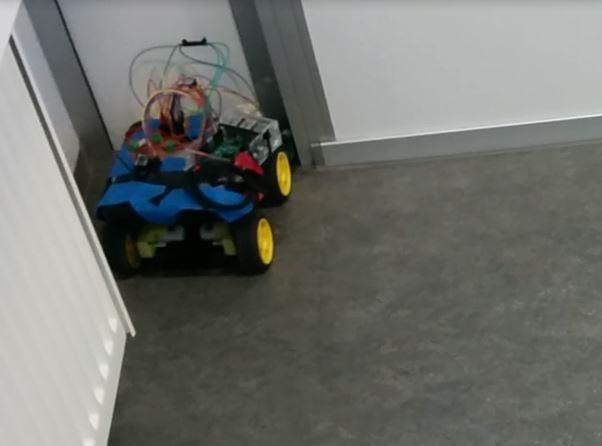
\includegraphics[width=\textwidth]{images/test-stuckincorner.jpg}
		\subcaption{Rover stuck in a corner}
		\label{corner}
	\end{subfigure}%
	\quad
	\begin{subfigure}[H]{0.4\textwidth}
		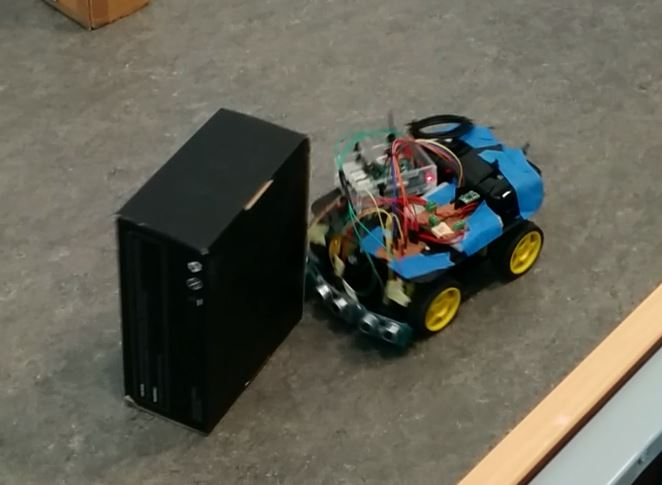
\includegraphics[width=\textwidth]{images/test-badmeasuringangle.jpg}
		\subcaption{Bad angle for measurements}
		\label{badangle}
	\end{subfigure}
\end{figure}

The current algorithm for the rover gets stuck in a loop if the rover drives directly into a corner(figure \ref{corner}). The reason for the looping is that the distance towards to wall of either side of the rover are equal, so it can not determine which direction it should steer towards.\\
Because of the skewed angles of the object in the test course, the rover would sometimes hit them. Figure \ref{badangle} clearly shows the rover hitting the object face on, because the ultrasonic sensors were not able to read the distance to the walls of the box because they are at a bad angle.

When the rover would turn to avoid objects or change its direction, it would skid across the floor. This resulted in the rover not turning on the spot, which reduces the accuracy of the steering.

\clearpage
\section{2D Mapping}

\subsection{Room test}
In order to test how well our mapping can keep the relation between objects, we made a small setup on a table.

\begin{figure}[H]
	\centering
	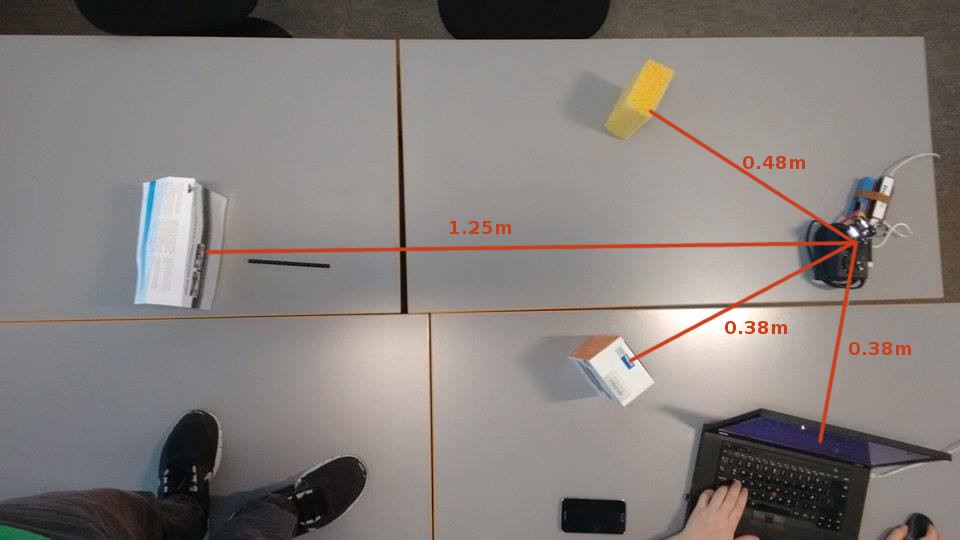
\includegraphics[scale=.4]{images/h101-photo.jpg}
	\caption{A photo of room H101 that was mapped.}
	\label{fig:internallidar}
\end{figure}
	
This figure shows what the setup was, with the addition of some distances.


\begin{figure}[H]
	\centering
	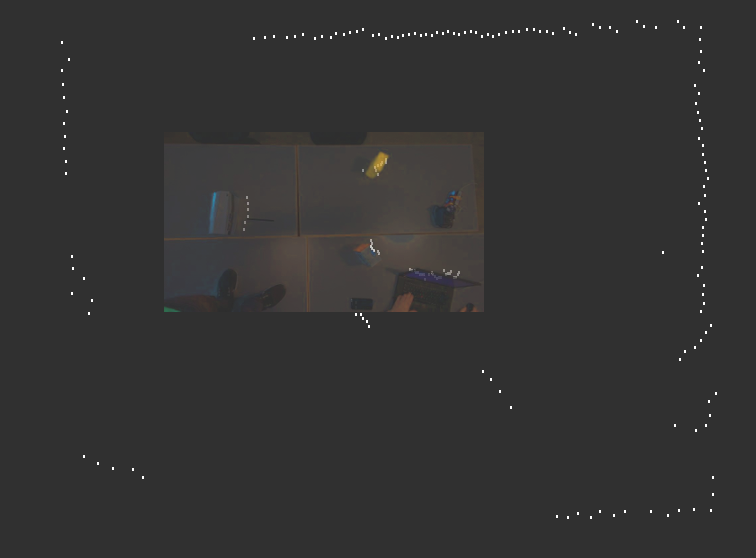
\includegraphics[scale=.4]{images/h101_obstacles_overlay.png}
	\caption{A map of room H101 with some small obstacles.}
	\label{fig:internallidar}
\end{figure}
	
This is the map that was generated by the laser, roughly overlayed with the picture of the setup.

Just from this very rough overlayed picture, it is easy to see that our map keeps the aspect-ratio of the physical world that it is mapping. 


\subsection{Hallway test}

Whatever

\begin{figure}
	content...
\end{figure}

\subsection{Outside test}
While running testing outside in areas with distances longer than 40 m the laser outputted a measurement of 255 cm. The reason behind this is that if the laser does not get a signal back it prints a error message with the integer 255. If that is not dealt with in the code the $/$scan topic will output a measurement of 2.55 m. We included a if statement that write 0 if a message with 255 is received. 

\begin{figure}[H]
	\centering
	\begin{subfigure}[H]{0.4\textwidth}
		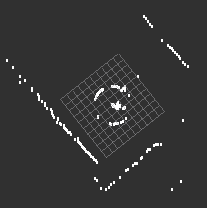
\includegraphics[width=\textwidth]{images/outside_error.png}
		\subcaption{}
		\label{}
	\end{subfigure}%
	\quad
	\begin{subfigure}[H]{0.5\textwidth}
		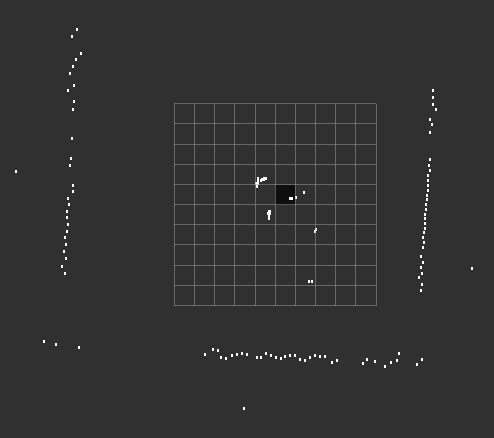
\includegraphics[width=\textwidth]{images/outside.png}
		\subcaption{}
		\label{}
	\end{subfigure}%
	\quad
\end{figure}